% ============================================================
%  Flusso di timbratura — sezione per tesi
%  Compilare con: pdflatex → biber → pdflatex × 2
%  Pacchetti richiesti: tikz, pgf-umlsd, listings, booktabs,
%                       geometry, hyperref, cleveref
% ============================================================

\section{Architettura e flusso del processo di timbratura}
\label{sec:flusso-timbratura}

Il nucleo funzionale del sistema è il processo di timbratura, attraverso
il quale un dipendente registra il proprio ingresso o la propria uscita
dalla sede lavorativa. Il processo è stato progettato con tre requisiti
fondamentali: \emph{assenza di interazione fisica} con il dispositivo di
stazione, \emph{verifica crittografica} dell'identità del dipendente e
\emph{validazione geografica} della posizione al momento della timbratura.

Il flusso coinvolge tre attori distinti: la \textbf{stazione} (un
dispositivo fisso, tipicamente un tablet, collocato all'ingresso della
sede), il \textbf{dipendente} (che utilizza il proprio dispositivo
personale dotato di sensore biometrico) e il \textbf{backend} (composto
da funzioni AWS Lambda e tabelle Amazon DynamoDB, descritto in dettaglio
nella sezione~\ref{sec:architettura}).

Il processo è strutturato in sette fasi sequenziali, illustrate nello
schema di Figura~\ref{fig:sequence-timbratura}.

% ── Figura: diagramma di sequenza ───────────────────────────────────────
\begin{figure}[ht]
\centering
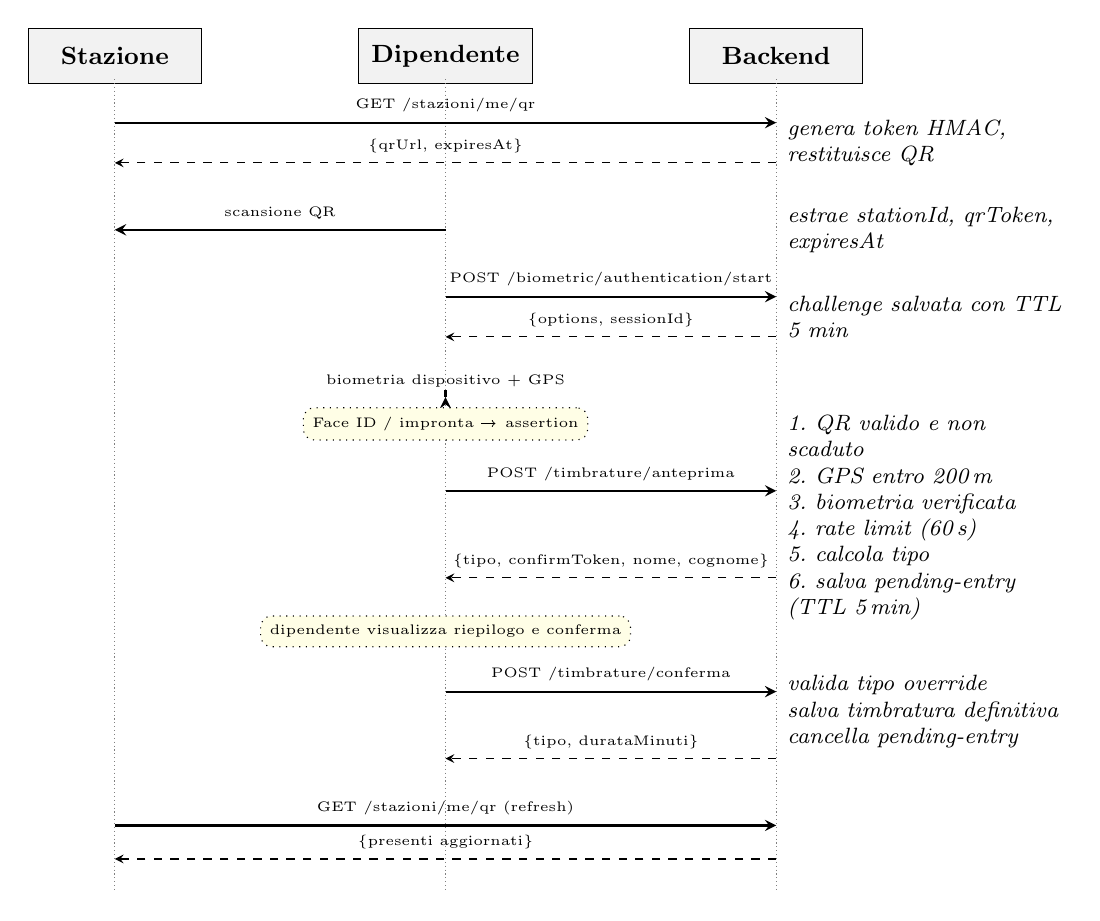
\begin{tikzpicture}[
    actor/.style={rectangle, draw, minimum width=2.2cm, minimum height=0.7cm,
                  fill=gray!10, font=\small\bfseries},
    msg/.style={->, >=stealth, thick},
    ret/.style={->, >=stealth, dashed},
    note/.style={font=\footnotesize\itshape, text width=3.5cm, align=left},
    timeline/.style={densely dotted, gray},
    x=4.2cm, y=-0.85cm
]

%% Attori
\node[actor] (sta) at (0,0) {Stazione};
\node[actor] (dip) at (1,0) {Dipendente};
\node[actor] (be)  at (2,0) {Backend};

%% Timeline
\foreach \x in {0,1,2} \draw[timeline] (\x,0.35) -- (\x,12.5);

%% Fase 1 — QR refresh
\draw[msg] (0,1) -- node[above,font=\tiny]{GET /stazioni/me/qr} (2,1);
\draw[ret] (2,1.6) -- node[above,font=\tiny]{\{qrUrl, expiresAt\}} (0,1.6);
\node[note] at (2.45,1.3) {genera token HMAC, restituisce QR};

%% Fase 2 — scansione
\draw[msg] (1,2.6) -- node[above,font=\tiny]{scansione QR} (0,2.6);
\node[note] at (2.45,2.6) {estrae stationId, qrToken, expiresAt};

%% Fase 3 — avvio biometria
\draw[msg] (1,3.6) -- node[above,font=\tiny]{POST /biometric/authentication/start} (2,3.6);
\draw[ret] (2,4.2) -- node[above,font=\tiny]{\{options, sessionId\}} (1,4.2);
\node[note] at (2.45,3.9) {challenge salvata con TTL 5 min};

%% Fase 4 — biometria + GPS
\draw[msg] (1,5.1) -- node[above,font=\tiny]{biometria dispositivo + GPS} (1,5.1);
\node[draw, dotted, rounded corners, font=\tiny, fill=yellow!10]
      at (1,5.5) {Face ID / impronta → assertion};

%% Fase 5 — anteprima
\draw[msg] (1,6.5) -- node[above,font=\tiny]{POST /timbrature/anteprima} (2,6.5);
\node[note] at (2.45,6.9)
      {1.\ QR valido e non scaduto\\
       2.\ GPS entro 200\,m\\
       3.\ biometria verificata\\
       4.\ rate limit (60\,s)\\
       5.\ calcola tipo\\
       6.\ salva pending-entry (TTL 5\,min)};
\draw[ret] (2,7.8) -- node[above,font=\tiny]{\{tipo, confirmToken, nome, cognome\}} (1,7.8);

%% Fase 6 — conferma utente
\node[draw, dotted, rounded corners, font=\tiny, fill=yellow!10]
      at (1,8.6) {dipendente visualizza riepilogo e conferma};

%% Fase 7 — conferma backend
\draw[msg] (1,9.5) -- node[above,font=\tiny]{POST /timbrature/conferma} (2,9.5);
\node[note] at (2.45,9.8)
      {valida tipo override\\
       salva timbratura definitiva\\
       cancella pending-entry};
\draw[ret] (2,10.5) -- node[above,font=\tiny]{\{tipo, durataMinuti\}} (1,10.5);

%% Fase 8 — aggiornamento stazione
\draw[msg] (0,11.5) -- node[above,font=\tiny]{GET /stazioni/me/qr (refresh)} (2,11.5);
\draw[ret] (2,12) -- node[above,font=\tiny]{\{presenti aggiornati\}} (0,12);

\end{tikzpicture}
\caption{Diagramma di sequenza del processo di timbratura.}
\label{fig:sequence-timbratura}
\end{figure}

% ── Fase 0 ───────────────────────────────────────────────────────────────
\subsection{Autenticazione della stazione}
\label{subsec:auth-stazione}

La stazione è un attore autonomo del sistema, distinto dagli utenti
Cognito. Al momento della messa in servizio, il responsabile crea la
stazione tramite il pannello di gestione; il backend genera
automaticamente un codice identificativo univoco nel formato
\texttt{STZ-XXXXXX} e restituisce le credenziali iniziali.

All'avvio, la stazione si autentica con una singola chiamata pubblica:

\begin{lstlisting}[language=,caption={Login della stazione.}]
POST /stazioni/login
{ "codice": "STZ-4A7F2B", "password": "..." }

→ 200 OK
{ "token": "<JWT HS256 24h>",
  "stazione": { "stationId", "descrizione", "codice" } }
\end{lstlisting}

Il token è un JWT firmato con algoritmo \textsc{HS256} e chiave segreta
condivisa, con scadenza di 24~ore. Viene conservato nel \texttt{localStorage}
del browser della stazione e allegato automaticamente, dall'interceptor
HTTP del frontend, a tutte le chiamate verso percorsi \texttt{/stazioni/me/*}.
La verifica avviene interamente lato Lambda, senza coinvolgere AWS Cognito.

% ── Fase 1 ───────────────────────────────────────────────────────────────
\subsection{Generazione e rotazione del codice QR}
\label{subsec:qr}

Il QR mostrato sullo schermo della stazione non è statico: viene
rigenerato ogni tre minuti mediante una chiamata periodica autenticata
con il JWT di stazione:

\begin{lstlisting}[language=,caption={Richiesta del codice QR.}]
GET /stazioni/me/qr
Authorization: Bearer <jwt-stazione>

→ 200 OK
{ "qrUrl": "https://app.example.com/timbratura?s=...&t=...&exp=...",
  "expiresAt": 1746482400,
  "presenti": 3,
  "ultimaTimbratura": { ... } }
\end{lstlisting}

Il campo \texttt{qrToken} incorporato nell'URL è calcolato come un
\textsc{HMAC-SHA256} della concatenazione di \texttt{stationId} e
\texttt{expiresAt}:

\[
  \mathtt{qrToken} = \mathrm{HMAC\text{-}SHA256}\!\left(k_{\mathrm{segreto}},\;
    \mathtt{stationId} \mathbin{\|} \texttt{":"} \mathbin{\|} \mathtt{expiresAt}
  \right)
\]

Questo approccio, noto come \emph{stateless token}, non richiede alcuna
persistenza lato server: al momento della verifica il backend ricalcola
l'HMAC con gli stessi parametri e confronta il risultato. La validità
temporale è garantita dal parametro \texttt{expiresAt}, controllato
esplicitamente prima della verifica crittografica.

% ── Fase 2 ───────────────────────────────────────────────────────────────
\subsection{Scansione del QR e validazione preliminare}
\label{subsec:scansione}

Il dipendente inquadra il QR con il proprio dispositivo. Il browser
apre il componente \texttt{TimbratureComponent}, che estrae i tre
parametri dall'URL (\texttt{s}, \texttt{t}, \texttt{exp}) ed esegue
immediatamente una verifica di scadenza lato client:

\begin{lstlisting}[language=TypeScript,caption={Verifica scadenza QR lato frontend.}]
if (Math.floor(Date.now() / 1000) > this.expiresAt) {
  this.errore = 'QR scaduto — chiedi alla stazione di aggiornarlo';
  return;
}
\end{lstlisting}

Questo controllo riduce le chiamate al backend nel caso più comune
(QR non aggiornato), ma non sostituisce la verifica server-side, che
rimane autoritativa.

% ── Fase 3 ───────────────────────────────────────────────────────────────
\subsection{Inizializzazione dell'autenticazione biometrica}
\label{subsec:biometria-start}

Il sistema adotta il protocollo \textsc{WebAuthn} (Web Authentication
API, standard \textsc{W3C}) per la verifica biometrica. Il processo
inizia con una chiamata pubblica, non autenticata, che restituisce la
\emph{challenge} crittografica necessaria al dispositivo:

\begin{lstlisting}[language=,caption={Avvio dell'autenticazione biometrica.}]
POST /biometric/authentication/start

→ 200 OK
{ "options": { "challenge": "<base64url>",
               "rpId": "app.example.com",
               "allowCredentials": [...],
               "timeout": 60000 },
  "sessionId": "<uuid>" }
\end{lstlisting}

Il backend genera la challenge casualmente, la salva nella tabella
\texttt{WebAuthnCredentials} con un TTL di cinque minuti e associa la
voce al \texttt{sessionId}. Quest'ultimo viene restituito al client per
collegare questa fase alla successiva chiamata \texttt{/anteprima}.

% ── Fase 4 ───────────────────────────────────────────────────────────────
\subsection{Autenticazione biometrica sul dispositivo}
\label{subsec:biometria-device}

Le \texttt{options} ricevute vengono passate alla libreria
\texttt{@simplewebauthn/browser}, che invoca l'API nativa del sistema
operativo:

\begin{lstlisting}[language=TypeScript,caption={Esecuzione della biometria lato client.}]
const assertion = await startAuthentication(options);
\end{lstlisting}

Il sistema operativo presenta all'utente il meccanismo di sblocco
configurato sul dispositivo (Face ID, impronta digitale, PIN di
sistema). In caso di autenticazione positiva, la libreria produce un
oggetto \texttt{assertion} contenente la risposta firmata con la chiave
privata del dispositivo. La proprietà fondamentale del protocollo
\textsc{WebAuthn} è che la chiave privata non lascia mai il dispositivo:
il backend verifica l'identità confrontando la firma con la chiave
pubblica precedentemente registrata, senza mai avere accesso al segreto.

In parallelo all'autenticazione biometrica, il frontend richiede la
posizione \textsc{GPS} del dispositivo con un timeout di otto secondi.
L'acquisizione del segnale non è bloccante: se non disponibile entro
il limite, il flusso prosegue e sarà il backend a decidere se rifiutare
la richiesta in base alla configurazione della stazione.

% ── Fase 5 ───────────────────────────────────────────────────────────────
\subsection{Fase di anteprima: verifica e calcolo del tipo}
\label{subsec:anteprima}

L'endpoint \texttt{POST /timbrature/anteprima} costituisce il nucleo
verificativo del sistema. Riceve in ingresso tutti gli elementi raccolti
nelle fasi precedenti ed esegue cinque controlli in sequenza, ciascuno
dei quali può interrompere il flusso con un codice di errore specifico.

\begin{lstlisting}[language=,caption={Payload della chiamata di anteprima.}]
POST /timbrature/anteprima
{ "stationId":  "uuid",
  "qrToken":    "hex-hmac",
  "expiresAt":  1746482400,
  "assertion":  { ...webauthn... },
  "sessionId":  "uuid",
  "lat":        45.4654,
  "lng":        9.1866 }
\end{lstlisting}

\paragraph{1. Validità temporale del QR.}
Il backend verifica che il timestamp corrente sia precedente a
\texttt{expiresAt}. Questa verifica è duplicata rispetto al controllo
client-side per prevenire attacchi in cui il QR viene catturato e
riutilizzato dopo la scadenza.

\paragraph{2. Autenticità del QR.}
Il backend ricalcola il token \textsc{HMAC} con gli stessi parametri
e confronta il risultato con il \texttt{qrToken} ricevuto. Un esito
negativo indica che il token è stato alterato o è destinato a una
stazione diversa.

\paragraph{3. Validazione geografica.}
Se la stazione ha coordinate \textsc{GPS} registrate, il backend
calcola la distanza tra la posizione del dipendente e la stazione
tramite la formula di Haversine~\eqref{eq:haversine}. Se la distanza
supera i 200 metri, la richiesta viene rifiutata.

\begin{equation}
  d = 2R \arctan\!\left(
    \sqrt{a},\, \sqrt{1-a}
  \right), \quad
  a = \sin^2\!\frac{\Delta\phi}{2}
    + \cos\phi_1 \cos\phi_2 \sin^2\!\frac{\Delta\lambda}{2}
  \label{eq:haversine}
\end{equation}

dove $R = 6\,371\,000$~m è il raggio terrestre, $\phi$ la latitudine
e $\lambda$ la longitudine in radianti.

\paragraph{4. Verifica biometrica.}
Il backend recupera la challenge associata al \texttt{sessionId},
verifica la firma dell'assertion con la chiave pubblica registrata
dell'utente tramite la libreria \texttt{@simplewebauthn/server} e
controlla il \emph{counter} WebAuthn, un valore monotonicamente
crescente che previene attacchi di tipo \emph{replay}. In caso di
successo, viene estratto il \texttt{userId} del dipendente.

\paragraph{5. Rate limiting.}
Per prevenire timbrature duplicate dovute a doppi click o errori
operativi, il backend recupera l'ultima timbratura dell'utente e
rifiuta la richiesta se è trascorso meno di 60 secondi.

\paragraph{Calcolo del tipo.}
Superate le cinque verifiche, il backend determina automaticamente se
la timbratura è un'entrata o un'uscita in base all'ultima registrazione
dell'utente, secondo la logica illustrata in
Tabella~\ref{tab:calcolo-tipo}.

\begin{table}[ht]
\centering
\caption{Logica di determinazione del tipo di timbratura.}
\label{tab:calcolo-tipo}
\begin{tabular}{lll}
\toprule
\textbf{Condizione} & \textbf{Tipo calcolato} & \textbf{Motivazione} \\
\midrule
Nessuna timbratura precedente  & entrata & primo accesso \\
Ultima era uscita              & entrata & turno concluso \\
Ultima entrata $< 20$ ore fa   & uscita  & turno in corso \\
Ultima entrata $\geq 20$ ore fa & entrata & uscita dimenticata \\
\bottomrule
\end{tabular}
\end{table}

La soglia di 20 ore è stata scelta per coprire i turni notturni
(massimo 12 ore) preservando un margine sufficiente a rilevare le
uscite dimenticate, che statisticamente si manifestano dopo un'intera
giornata lavorativa.

\paragraph{Pending-entry.}
Completate le verifiche, il backend non salva ancora la timbratura
definitiva, ma inserisce una \emph{pending-entry} nella tabella
\texttt{Timbrature} con una chiave primaria sintetica:

\begin{lstlisting}[language=,caption={Struttura della pending-entry.}]
{
  "userId":    "pending#<confirmToken>",
  "timestamp": "2026-05-05T08:22:10.000Z",
  "realUserId": "<uuid-dipendente>",
  "tipo": "uscita",
  "expiresAt": 1746482730    /* adesso + 300 secondi — TTL DynamoDB */
}
\end{lstlisting}

L'utilizzo di un prefisso \texttt{pending\#} permette di filtrare
queste voci nelle query sui dati reali. Il campo \texttt{expiresAt}
è configurato come attributo \textsc{TTL} della tabella DynamoDB:
le voci scadute vengono eliminate automaticamente dal servizio entro
pochi minuti dalla scadenza, senza richiedere alcun processo di pulizia
applicativo.

% ── Fase 6-7 ─────────────────────────────────────────────────────────────
\subsection{Fase di conferma: persistenza e override}
\label{subsec:conferma}

Ricevuta la risposta di anteprima, il frontend visualizza il riepilogo
al dipendente: nome, cognome e tipo di timbratura calcolato. È prevista
la possibilità di invertire il tipo prima della conferma, per gestire
situazioni eccezionali come i turni notturni a cavallo della mezzanotte.

La conferma viene inviata con:

\begin{lstlisting}[language=,caption={Payload della conferma.}]
POST /timbrature/conferma
{ "confirmToken": "<hex>",
  "tipoOverride": "entrata"   /* opzionale */ }
\end{lstlisting}

Il backend recupera la pending-entry tramite il \texttt{confirmToken},
ne verifica la scadenza e, se è presente un \texttt{tipoOverride},
ri-verifica la coerenza della sequenza prima di accettarlo. Questa
seconda verifica impedisce che un override produca sequenze illogiche
(due entrate consecutive o due uscite consecutive), che potrebbero
corrompere il calcolo delle ore lavorate.

La timbratura definitiva viene quindi scritta nella tabella
\texttt{Timbrature} con il \texttt{userId} reale del dipendente e la
pending-entry viene immediatamente cancellata. La data viene calcolata
in ora locale italiana tramite la libreria Luxon, indipendentemente dal
fuso orario UTC del timestamp di sistema, per garantire il corretto
raggruppamento delle timbrature notturne a cavallo della mezzanotte:

\begin{lstlisting}[language=TypeScript,caption={Calcolo della data locale.}]
import { DateTime } from 'luxon';

const data = DateTime.now()
  .setZone('Europe/Rome')
  .toFormat('yyyy-MM-dd');
\end{lstlisting}

Se la timbratura è un'uscita, il backend calcola la durata del turno
cercando l'ultima entrata dello stesso utente alla stessa stazione e
la restituisce al frontend espressa in minuti.

% ── Sicurezza ─────────────────────────────────────────────────────────────
\subsection{Considerazioni sulla sicurezza}
\label{subsec:sicurezza-timbratura}

Il processo descritto presenta diverse proprietà di sicurezza rilevanti.

\textbf{Separazione delle responsabilità.} Il QR viene generato dalla
stazione autenticata; la biometria viene verificata lato server tramite
chiave pubblica; la posizione geografica è controllata server-side. Nessun
singolo elemento, se compromesso, è sufficiente a completare una
timbratura fraudolenta.

\textbf{Assenza di stato condiviso tra le fasi.} Le due chiamate
(\texttt{/anteprima} e \texttt{/conferma}) non richiedono sessioni HTTP:
il collegamento avviene tramite il \texttt{confirmToken}, un valore
casuale a 128 bit generato server-side e trasmesso cifrato su \textsc{TLS}.

\textbf{Validità temporale multipla.} Esistono tre livelli di scadenza
indipendenti: il QR (3 minuti), la challenge biometrica (5 minuti) e la
pending-entry (5 minuti). La compromissione di uno solo di questi
elementi non consente di completare il flusso.

\textbf{Protezione replay.} Il counter WebAuthn impedisce il riutilizzo
di una assertion catturata; il rate limiting di 60 secondi impedisce la
doppia timbratura; la pending-entry viene cancellata atomicamente al
momento della conferma, rendendola inutilizzabile una seconda volta.
